% resDoc.tex

\documentclass[11pt]{book}\usepackage[]{graphicx}\usepackage[]{color}
%% maxwidth is the original width if it is less than linewidth
%% otherwise use linewidth (to make sure the graphics do not exceed the margin)
\makeatletter
\def\maxwidth{ %
  \ifdim\Gin@nat@width>\linewidth
    \linewidth
  \else
    \Gin@nat@width
  \fi
}
\makeatother

\definecolor{fgcolor}{rgb}{0.345, 0.345, 0.345}
\newcommand{\hlnum}[1]{\textcolor[rgb]{0.686,0.059,0.569}{#1}}%
\newcommand{\hlstr}[1]{\textcolor[rgb]{0.192,0.494,0.8}{#1}}%
\newcommand{\hlcom}[1]{\textcolor[rgb]{0.678,0.584,0.686}{\textit{#1}}}%
\newcommand{\hlopt}[1]{\textcolor[rgb]{0,0,0}{#1}}%
\newcommand{\hlstd}[1]{\textcolor[rgb]{0.345,0.345,0.345}{#1}}%
\newcommand{\hlkwa}[1]{\textcolor[rgb]{0.161,0.373,0.58}{\textbf{#1}}}%
\newcommand{\hlkwb}[1]{\textcolor[rgb]{0.69,0.353,0.396}{#1}}%
\newcommand{\hlkwc}[1]{\textcolor[rgb]{0.333,0.667,0.333}{#1}}%
\newcommand{\hlkwd}[1]{\textcolor[rgb]{0.737,0.353,0.396}{\textbf{#1}}}%

\usepackage{framed}
\makeatletter
\newenvironment{kframe}{%
 \def\at@end@of@kframe{}%
 \ifinner\ifhmode%
  \def\at@end@of@kframe{\end{minipage}}%
  \begin{minipage}{\columnwidth}%
 \fi\fi%
 \def\FrameCommand##1{\hskip\@totalleftmargin \hskip-\fboxsep
 \colorbox{shadecolor}{##1}\hskip-\fboxsep
     % There is no \\@totalrightmargin, so:
     \hskip-\linewidth \hskip-\@totalleftmargin \hskip\columnwidth}%
 \MakeFramed {\advance\hsize-\width
   \@totalleftmargin\z@ \linewidth\hsize
   \@setminipage}}%
 {\par\unskip\endMakeFramed%
 \at@end@of@kframe}
\makeatother

\definecolor{shadecolor}{rgb}{.97, .97, .97}
\definecolor{messagecolor}{rgb}{0, 0, 0}
\definecolor{warningcolor}{rgb}{1, 0, 1}
\definecolor{errorcolor}{rgb}{1, 0, 0}
\newenvironment{knitrout}{}{} % an empty environment to be redefined in TeX

\usepackage{alltt}
\usepackage{resDocSty}
\usepackage{appendix}
\usepackage{cite}

\usepackage{longtable,array}   % need array when specifying a ragged right column:  >{\raggedright\arraybackslash}{p2in}.
% \renewcommand{\chaptername}{Appendix}
% \renewcommand*{\chaptername}{Appendix}
% \addto\captionsenglish{\renewcommand\chaptername{Part}}
\usepackage{import}            % for figures in chapter subdirectories
%\usepackage{float}             % Allow figures and tables to be controlled better (avoid the floating).

% Had these for YMR Eqns appendix:
% \renewcommand{\footrulewidth}{0.4pt}
% \renewcommand{\headrulewidth}{0pt}

% For appendices:
\usepackage{graphicx}          % For inclusion of figures
\usepackage{verbatim,fancyvrb} % Check - may be in .sty file
\usepackage{xifthen}           % provides \ifthenelse and \isempty
\usepackage{color, colortbl}
\usepackage{arydshln}          % For dashed lines in tables (has to be loaded after other stuff)
\usepackage{pdfpages}          % So we can import PDFs into the document (e.g. request for science advice).

% For hyperlinked references (figures and citations, etc.). The bookmarksdepthlevel allows
%  the TOC to be shown in the bookmarks tree in the output PDF.
\usepackage[bookmarks,bookmarksopen,bookmarksdepth=4]{hyperref}
\hypersetup{                   % Set up the hyperref options here
    pdftitle={Arrowtooth Flounder},
    pdfauthor={Chris Grandin},
    pdfsubject={Stock Assessment},
    %pdfkeywords={keyword1, keyword2},
    bookmarksnumbered=true,
    bookmarksopen=true,
    bookmarksopenlevel=1,
    colorlinks=true,
    linkcolor=blue,
    allcolors=blue,
    citecolor=cyan,
    pdfstartview=Fit,
    pdfpagemode=UseOutlines
    %pdfpagelayout=TwoPageRight
}
% Use the following codes for references within the document.
%   chap: chapter
%    sec: section
% subsec: subsection
%    fig: figure
%    tab: table
%     eq: equation
%    lst: code listing
%    itm: enumerated list item
%    app: appendix subsection
\usepackage{hypcap}            % So links will anchor at figure, not caption

\usepackage{subfig}            % For two-panel plots
\usepackage{scrextend}         % For indenting blocks of text with 'addmargin'
\usepackage{relsize}           % For mathlarger, which makes equations bigger
%\usepackage{mathtools}        % For mathmboxes for use in the equations appendix
\usepackage{algorithm}         % For display of pseudocode
\usepackage{algpseudocode}     % For display of pseudocode
\usepackage{linegoal}          % For display of pseudocode
% A \Let command for defining assignments within the algorithmic environment which
% supports automatic indentation when the second argument is too long to fit
% on one line
\newcommand*{\Let}[2]{\State #1 $\gets$
\parbox[t]{\linegoal}{#2\strut}}
% A \State command that supports automatic indentation when the argument's
% content is too long to fit on one line
\newcommand*{\LongState}[1]{\State
\parbox[t]{\linegoal}{#1\strut}}

\usepackage{enumitem}          % To remove spacing between list items [noitemsep,nolistsep]
\newlist{longitem}{enumerate}{5}
\setlist[longitem,1]{label=\arabic*)}
\setlist[longitem,2]{label=\alph*)}
\setlist[longitem,3]{label=\roman*)}
\setlist[longitem,4]{label=\arabic*)}
\setlist[longitem,5]{label=\alph*)}

\definecolor{rowclr}{RGB}{255, 192, 203}
\newcommand{\sQuote}[1]{`#1'}
\newcommand{\dQuote}[1]{``#1''}
\newcommand{\eqn}[1]{\begin{equation}#1\end{equation}}
\newcommand{\gfrac}[2]{\genfrac{}{}{}{0}{#1}{#2}}

\newcommand\bestfig[6]{ % #1=filename, #2=main caption, #3=figure height, #4=short caption #5=file extension #6=directory
	% needs package epstopdf to work
	\begin{figure}[htpb] %[htbp]
	\centering
	\ifthenelse{ \isempty{#5} \OR \equal{#5}{eps} }
		{\includegraphics[width=6.5in,height=#3in,keepaspectratio=TRUE]{#6#1.eps}}
		{\setlength\fboxsep{0pt}
		 \setlength\fboxrule{0pt}
		 \fbox{\includegraphics[width=6.5in,height=#3in,keepaspectratio=TRUE]{#6#1.#5}}}
	% source: http://xelatex.blogspot.ca/2008/03/newcommand-with-optional-argument.html
	\ifthenelse{\isempty{#4}}
		{\caption[#2]{#2}}  % \vspace{-2ex}} AME removing
		{\caption[#4]{#2}}  % \vspace{-2ex}}  ``
	\label{fig:#1}
	\end{figure}
        }

\newcommand\pbsfig[5]{    % #1=filename, #2=main caption, #3=figure height, #4=short caption, #5=directory
	\begin{figure}[tp] %[htbp]  Rowan had ht!
	\centering
	\includegraphics[width=6.5in,height=#3in,keepaspectratio=TRUE]{#5#1.eps}
	% source: http://xelatex.blogspot.ca/2008/03/newcommand-with-optional-argument.html
	\ifthenelse{\isempty{#4}}
		{\caption[#2]{#2}\vspace{-2ex}}
		{\caption[#4]{#2}\vspace{-2ex}}
	\label{fig:#1}
	\end{figure}
	%\clearpage
}

% eor - Show two things with a vertical bar between them
\newcommand{\eor}[2]{{#1$\Vert$#2}}
% bM - makes equations larger
\newcommand{\bM}[1]{\mathlarger{\mathlarger{#1}}}
% Allow newline breaks in a table cell: syntax is \specialcell{first line\\secondline}
\newcommand{\specialcell}[2][c]{\begin{tabular}[#1]{@{}c@{}}#2\end{tabular}}

\newcommand{\fishname}{Arrowtooth Flounder}
% sciencename - Science name for the species being assessed
\newcommand{\sciencename}{Atheresthes stomias}

% Headers and footers
% For Res Doc, best to have a left and a right footer
%  (and/or header), not just one (for double-sided printing).
%
% \lhead{DRAFT -- Non-citable working paper}  % Omit for final ResDoc.
\lhead{}
\rhead{}
\lfoot{\fishname}           % Species common name for left footer
\rfoot{Coastwide}           % The area of the assessment for right footer
%\rfoot{WP 2012/P02a}       % Change to appendix number for appendices
                            % Will probably delete footers in main text
                            %  for final Res Doc.

% \linenumbers              % uncomment to add in line numbers
% \modulolinenumbers[5]     % just number every 5th line

% \def\AppLet{F}            % Appendix letter - we had this
                            %  to number equations in Appendix
                            %  F as (F.17) etc.
% \def\StartP{102}          % page start

\newcommand{\Bmsy}{B_\mathrm{MSY}}
\newcommand{\umsy}{u_\mathrm{MSY}}
\newcommand{\MapData}{C:/Work/ArrowtoothFlounder/2014Assessment/data/MapData}

\newcommand{\EstM}{`Estimate \emph{M}'}
\newcommand{\FixM}{`Fix \emph{M}'}
\IfFileExists{upquote.sty}{\usepackage{upquote}}{}

\begin{document}

\def \KnitrHomePath {C:/github/csas-latex/doc}
% Load iscam-gui list object scenarios - Make sure all are set up in correct order before running this
% Also, set up standard plot sizes for the document



% preamble.tex - Tables of Contents, Figures, Tables, plus Abstract
%  Useful to comment out when don't need all that (e.g. working on an
%  Appendix).

%%CoverPage
%\input{./csasCoverPage} - currently using word->pdf and merging pdfs
%  for ResDocs.
%\newpage
% For working paper, use this before using Word for actual submission.

% From Matt Grinnel's Tech Report document.
%\setlength{\parindent}{0mm}
\thispagestyle{fancyplain}
%\pagecolor{Tan}

\pagenumbering{roman}

\begin{flushleft}
\LARGE \textbf{Arrowtooth Flounder ({\bf \emph{Atheresthes stomias}}) stock assessment for the west coast of British Columbia}

% \TRtitleCap}
\end{flushleft}
\vfill
{\Large Chris Grandin, Robyn Forrest, and Paul J. Starr}
\vfill
% \TRaddy
\vfill
% \TRyear
\vfill
{\LARGE \textbf{Working paper number 2014/ARF01}}\\
 % Canadian Technical Report of\\Fisheries and Aquatic Sciences  \TRreportNumber}
\vspace{2cm}
[Replace with Word template for submission]
\vfill
% \lfoot{\includegraphics[height=5mm]{doc/DFOleft.jpeg}}
% \cfoot{}
% \rfoot{\includegraphics[height=5mm]{doc/DFOright.png}}
\clearpage

%% ---------------------------------------------------------------------

%%TOC will go here (page iii - req'mt by CSAS)
% \setcounter{page}{3}
\renewcommand{\contentsname}{\bf \large \vspace{-25mm} TABLE OF CONTENTS}
\addtocontents{toc}{\protect\thispagestyle{fancy}}
% \renewcommand{\cftchapterfont}{APPENDIX }\setlength{\cftfignumwidth}{1.5em}     % - ask Jaclyn, want to make it same as others.
%\begin{center}
%\tableofcontents
%\end{center}
%\newpage

% \nonumsection*{TABLE OF CONTENTS}

\begin{center}
\tableofcontents
\end{center}
\newpage

% Use Word template for these and cover page (use final YMR).

% Andy not using:
% \addtocontents{lof}{\protect\thispagestyle{fancy}}
%\renewcommand{\listfigurename}{\bf \large \vspace{-25mm} LIST OF MAIN FIGURES}     % JC and AME decided to restrict to just main ones.
%\renewcommand{\cftfigfont}{Figure }\setlength{\cftfignumwidth}{1.5em}
%\begin{center}
%\listoffigures
%\end{center}
%\addcontentsline{toc}{section}{LIST OF MAIN FIGURES}
%\newpage

%\addtocontents{lot}{\protect\thispagestyle{fancy}}
%\renewcommand{\listtablename}{\bf \large \vspace{-25mm} LIST OF MAIN TABLES}
%\renewcommand{\cfttabfont}{Table }\setlength{\cfttabnumwidth}{1.5em}
%\begin{center}
%\listoftables
%\end{center}
%\addcontentsline{toc}{section}{LIST OF MAIN TABLES}
%\clearpage

\leftskip=3em	%%required to indent Citation below
\parindent=-3em

{\bf Correct citation for this publication:}

Non-citable Working Paper.	%%(req'mt by CSAS)

%Cleary, J.S. and Haist, V. 2012.****
%Stock Assessment and Management Advice for the British Columbia Pacific Herring Stocks: 2012 Assessment and 2013 Forecasts.
%DFO Can. Sci. Advis. Sec. Res. Doc. 2012/xxx. xii + 151 p.

%JSC: would be nice to automate roman and regular page numbers. Counter? See Matt Grinnell's Tech Report latex files.

\leftskip=0em	%% end Citation indent
\parindent=-0em

%% \section*{Abstract}\addcontentsline{toc}{section}{ABSTRACT}
%% \nonumsection is centered
%\nonumsection*{ABSTRACT}\addcontentsline{toc}{section}{ABSTRACT}

% \newpage	%French abstract must appear on new page

%% \section*{R\'esum\'e}\addcontentsline{toc}{section}{R\'ESUM\'E}
% \nonumsection*{R\'ESUM\'E}\addcontentsline{toc}{section}{R\'ESUM\'E}

% \addcontentsline{toc}{section}{R\'ESUM\'E}

% hareng de la C.-B. sont g\'er\'es en fonction de cinq zones de stocks principales et de deux zones secondaires. En cons\'equence, l'information sur les prises et celle provenant des relev\'es est recueillie de fa\c{c}on ind\'ependante pour les sept zones, et on formule des avis scientifiques pour chacune. On s'est servi de toutes les donn\'ees biologiques disponibles sur la ponte, la composition selon l'\^{a}ge et la taille des stocks reproducteurs ainsi que sur les pr\'el\`{e}vements de la p\^{e}che commerciale pour d\'eterminer les niveaux d'abondance actuels. Ces derni\`{e}res ann\'ees, des examinateurs externes ont sugg\'er\'e que d'importantes r\'evisions soient apport\'ees au cadre d'\'evaluation du hareng, y compris au mod\`{e}le des prises selon l'\^{a}ge. Nous pr\'esentons donc un nouveau mod�le statistique int\'egr\'e des prises selon l'\^{a}ge (iSCAM) pour estimer conjointement l'abondance des stocks de hareng du Pacifique et les points de r\'ef\'erence connexes (partie I). Ce mod\`{e}le comprend des essais de simulation pour d\'emontrer que le mod\`ele peut estimer tous les param\`{e}tres ainsi qu'une param\'etrisation du nouveau mod\`{e}le d�\'evaluation comme le pr\'ec\'edent mod\`{e}le d�\'evaluation (mod\`{e}le des prises de hareng selon l'\^{a}ge ou HCAM) pour que l�on puisse comparer les estimations des param\`{e}tres et les estimations de la biomasse du stock reproducteur (en utilisant les donn\'ees de 1951 \`{a}) 2010) entre l'ancien mod\`{e}le (HCAM) et le nouveau (ISCAM). La partie II de ce document refl\`{e}te le nouveau cadre d'\'evaluation avec des donn\'ees des cinq zones de stock principales et des deux zones secondaires. Finalement, nous pr\'esentons des estimations de la biomasse avant la p\^{e}che et un avis sur les prises fond\'e sur les tableaux sur les d\'ecisions qui utilisent les pr\'evisions du recrutement \`{a} l'\^{a}ge 3 faible, moyen et bon ainsi que sur les tableaux sur la probabilit\'e du risque afin d'\'eclairer la prise de d\'ecision.



              % Table of contents, etc.
% \setcounter{chapter}{0}
% \setcounter{table}{0}
% \setcounter{figure}{0}
\setcounter{secnumdepth}{3}    % To number subsubheadings-ish

% To number sections, tables etc. as 1, 2, 3, not 1.1 etc. (where
%  the first 1 would be chapter number).
\renewcommand{\thesection}{\arabic{section}}
\renewcommand{\thetable}{\arabic{table}}
\renewcommand{\thefigure}{\arabic{figure}}
\renewcommand{\theequation}{\arabic{equation}}

% \subimport{mainDoc/}{mainDocRev}

% mainDoc.tex - Main part of the document

\nonumsection*{ABSTRACT}\addcontentsline{toc}{section}{ABSTRACT}

\fishname (\emph{\sciencename}, Turbot) is an important component of the trawl fishery in British Columbia, and are caught ubiquitously along the west coast of British Columbia (Figure~\ref{fig:cpue}).

\newpage	%French abstract must appear on new page

% \section*{R\'esum\'e}\addcontentsline{toc}{section}{R\'ESUM\'E}
\nonumsection*{R\'ESUM\'E}\addcontentsline{toc}{section}{R\'ESUM\'E}

% \addcontentsline{toc}{section}{R\'ESUM\'E}

\clearpage

% Need numbering back to Arabic.
\pagenumbering{arabic}
\setcounter{page}{1}

\section{INTRODUCTION}

This stock assessment is for \fishname\ in combined Pacific Marine Fisheries Commission (PMFC) major areas 3CD and 5ABCDE off the west coast of British Columbia. \fishname\ make up a large component of the trawl fishery, but most are and have been discarded at sea. Proteolysis occurs in the muscle tissue of this species a short time after it is caught, which makes the flesh very mushy and unpalatable. There is a market in Korea for the frills, and a market for the fillets if they are frozen at sea, very shortly after capture.

\subsection{PURPOSE OF DOCUMENT}

This document provides stock assessment advice to fisheries managers for Arrowtooth Flounder. This advice was requested by the Groundfish Management Unit (GMU) of the DFO Pacific Region (Appendix A), which specified that the advice be framed in terms of the DFO Sustainable Fisheries Framework (SFF) (see \citet{dfo09}). This advice is presented as a set of decision tables that provide probabilities of exceeding reference points over a range of projection years and across a range of constant catch scenarios (without feedback controls). Reference points are defined below.

CITETEST: \citet{arf1995}, \citet{arf1999a}, \citet{arf1999b}, \citet{arf2000}, \citet{arf2001}, \citet{arf2003}, \citet{arf2006},\citet{arf2013}.

\subsection{BIOLOGICAL BACKGROUND}

Arrowtooth Flounder (\emph{Atheresthes stomias}, Turbot) is a species of flatfish found along the rim of the Northeast Pacific Ocean. The most distinguishing feature of Arrowtooth Flounder is its large teeth, for which it was named. As juveniles smaller than ~380mm, Arrowtooth Flounder are monomorphic. After maturing, they are sexually dimorphic with adult females being larger than males (Appendix~\ref{chap:biological}, Figure~\ref{fig:vonb}).

\subsection{RANGE AND DISTRIBUTION}


\subsection{OVERVIEW OF FISHERY}


\section{ASSESSMENT BOUNDARIES AND BACKGROUND}

For this assessment, we use PMFC major areas 3CD and 5ABCDE, covering almost all of the west coast of Vancouver Island (Figure~\ref{fig:areas}).

Advice for managers was requested to be guided by the DFO Sustainable Fisheries Framework, particularly the Fishery Decision-making Framework Incorporating the Precautionary Approach. Consequently, advice to managers is presented as a set of decision tables that provide probabilities of exceeding reference points for various years of projections across a range of constant catch scenarios.

A DFO Technical Working Group provided valuable guidance with respect to many of the decisions that were made in the course of this work.

\section{CATCH DATA}
*Table with history of quota and catch from 1996-present

\section{FISHERIES MANAGEMENT}

\clearpage

\section{SURVEY DESCRIPTIONS}

Six sets of fishery independent survey indices of abundance were used:

\begin{enumerate}[noitemsep,nolistsep]
  \item the West Coast Vancouver Island Synoptic Survey series, from 2004-2014 (even years only), referred to here as the `WCVISS series'.
  \item the Hecate Strait Synoptic Survey series, from 2005-2013 (odd years only), referred to here as the `HSSS series'.
  \item the Hecate Strait Multispecies Assemblage Survey, for 1996, 1998, 2000, 2002, and 2003, referred to here as `HSMAS'.
  \item the Queen Charlotte Sound Synoptic Survey, from 2003-2013 (odd years only), referred to here as `QCSSS'.
  \item the West Coast Vancouver Island Shrimp Trawl Survey, from 1996-2014 (all years), referred to here as `WCVISTS'.
  \item the Queen Charlotte Sound Shrimp Trawl Survey, from 1999-2013 (all years), referred to here as `QCSSTS'.
\end{enumerate}

The suitability of each survey was examined (Table~\ref{tab:surveySuitability}). The WCVISS, HSSS, HSMSAS, and QCSSS were all designed to produce indices for the demersal fish species of the Northeast Pacific, and the two shrimp trawl surveys WCVISTS and QCSSTS were designed to generate shrimp indices. The depth ranges differ by a large amount, with the 4 groundfish surveys having ranges from 18 m to 660 m. The shrimp trawl surveys have a maximum depth of 251 m and 305 m for the WCVISTS and QCSSTS respectively (Table~\ref{tab:surveySuitability}). The depth range for \fishname\ is 50 m to 900 m (\citet{arf2001}); the shrimp trawl surveys cover much less of the habitable depth range than the groundfish surveys do, 

suggesting that they might not be suitable as an index of stock for

The relative biomass survey indices are used as data in the model along with the associated relative error for each index value.

Pre-1996 commercial catch and effort data were also investigated with the intent of creating CPUE-based abundance indices for use in the stock assessment model. This approach was abandoned because it was felt that there were problems with the reliability of the data as well as questions as to the representative nature of the resulting indices, given the schooling behaviour of the species and the capacity of fishers to target these schools. Given the concern that the resulting indices would be hyperstable, they were not used in this assessment.

\clearpage

\section{BIOLOGICAL INFORMATION}

\subsection{BIOLOGICAL SAMPLES}

\subsection{GROWTH PARAMETERS}

\subsection{MATURITY}

\subsection{NATURAL MORTALITY}

PAST ASSESSMENTS have assumed M.... etc.. cite Fargo Starr and Alaska center assessments. Very sensitive to assumptions in the model iscam.

Male and female natural mortalities were estimated as parameters of the model (see Appendix~F), using an informed prior based on the marginal posterior distributions from the QCS POP assessment , specifically a normal prior with mean 0.07 and standard deviation 0.007 for both sexes (see Appendix~F). The QCS assessment used a prior based on a POP assessment for the Gulf of Alaska , with mean 0.06 and standard deviation 0.006.

In recent assessments , model runs that fixed natural mortality were also used to provide the final advice to managers. However, because we were able to develop a prior based on Canadian POP data, and since the resulting Bayesian estimates of natural mortality and steepness (defined below) are uncorrelated (Appendix~G), only runs that estimate natural mortality are used in this assessment (as agreed upon by the Technical Working Group). Prior distributions for all estimated parameters are given in Table F.4.

\section{AGE-STRUCTURED MODEL}

We attempted a two-sex, age-structured stochastic model to reconstruct the population trajectory of Arrowtooth Flounder
*Reference Appendix for model outputs and sensitivities...

REASONS model was rejected.

\section{RESULTS}

MOVE TO APPENDIX FOR MODEL RESULTS
THIS IS ALL POP!!!!!!!!!!!!!!!!!!!!!!!!!!
The base case model run had credible fits to the data, as demonstrated by visual examination of the MPD fits and the patterns of residuals (results in Appendix G). The MCMC results showed satisfactory convergence of the MCMC search process (Appendix G). Priors and marginal posteriors of the estimated parameters are also given in Appendix G, along with the values of the estimated parameters (Table \ref{tab:MCMCpar}). For example, natural mortality is estimated as having median (and 5-95\% credible interval) of 0.069~(0.060-0.079) for females and 0.072~(0.063-0.082) for males. Steepness is estimated to be 0.70~(0.48-0.91). The remaining MCMC results, of more general interest, are given here.

Figure \ref{fig:VBcatch} shows the MCMC results for the estimated vulnerable biomass, together with the reconstructed historical catches, and Figure \ref{fig:BVBnorm} shows the estimated medians of vulnerable and spawning (mature females only) biomass relative to their unfished values. (The full MCMC results for spawning biomass are included later in Figure \ref{fig:Bproj} regarding projections). These demonstrate a slight decline in biomass from 1940 to 1960 with the onset of fishing, followed by a very sharp decline in the 1960s due to heavy fishing (primarily by foreign fleets). After the cessation of foreign fishing, the biomass increased through the remainder of the 1970s. The biomass then declined through the 1980s until the mid-1990s, and has since increased, with median values of relative biomass now above the 1980 values.

Estimates of various quantities of interest are given in Table \ref{tab:MCMCderived}. In particular, the median (and 5-95\% credible interval) for $B_{2013}/B_0$, the ratio of current spawning biomass ($B_{2013}$) to the unfished equilibrium level ($B_0$), is 0.41~(0.19-0.68); thus 0.41 is the value for the final circle in Figure \ref{fig:BVBnorm}.
% (This ratio is sometimes known as depletion).

The estimated recruitments (age-1 fish, Figure \ref{fig:recruitsMCMC}) in part further explain the aforementioned stock trajectory. There was lower-than-average recruitment in the early 1970s, which may, together with increased catches, explain why the vulnerable biomass declined through the 1980s (note the approximate ten-year lag from recruitment to fish becoming fully selected by the commercial fishery). There are a number of year classes with approximately double the long-term average recruitment. This is unlike the patterns observed for the QCS area 5ABC stock (Figure 5 of  and the companion assessment for area 5DE , which both exhibited a dominant 1976 year class (age-1 recruits in 1977) that was approximately five times larger than the long-term average recruitment.

Figure \ref{fig:exploitMCMC} shows the estimated exploitation rates (ratio of total catch to the vulnerable biomass in the middle of the year), which peaked in the mid-1960s due to the large foreign catches, and then peaked again (although not as high) in the early 1990s due to increased domestic exploitation. Exploitation rates have remained low since the mid-1990s, with $u_{2012}$, the exploitation rate for 2012, estimated to be 0.035~(0.018-0.077).

Estimates of further quantities of interest, such as absolute values of biomass (rather than relative values), are also given in Table \ref{tab:MCMCderived}, as well as quantities based on MSY, discussed below.

\section{RECCOMENDATIONS AND YIELD OPTIONS}

\subsection{CURRENT STOCK LEVEL}

\subsection{REFERENCE POINTS}

\subsection{PROJECTION RESULTS AND DECISION TABLES}

\section{GENERAL COMMENTS}

\section{FUTURE RESEARCH AND DATA REQUIREMENTS}

\section{ACKNOWLEDGEMENTS}

We thank the members of the Arrowtooth Flounder Technical Working Group (Rowan Haigh, Kendra Holt, Rob Kronlund, Barry Ackerman, Greg Workman) for their valuable advice as this project progressed. We thank participants of the Regional Peer Review meeting for their comments at the meeting, and Rowan Haigh for chairing. We especially thank James Thorsen (NOAA) and Joanne Morgan (DFO) for their written reviews of the working paper. We also thank Steve Wischniowski and the members of the Sclerochronology Laboratory at the Pacific Biological Station for their processing of over 6,000 Arrowtooth Flounder otoliths in 2014.

\addcontentsline{toc}{section}{BIBLIOGRAPHY}
\bibliographystyle{resDoc}
\bibliography{../../all}

\clearpage

\begin{figure}[htp]
\begin{center}
\includegraphics[width=6in,keepaspectratio=true]{cpueFigures/ARF-1996-2014-CPUE.eps}
\end{center}
\vspace{0mm}
% To get the grid size in km^2 for the caption:
% While in the gui for the map, type mean(xtcall(PBSmap)$pdata$area) for the map you currently have loaded.
\caption{Mean catch-per-unit-effort (CPUE, kg/h) of Arrowtooth Flounder in grid cells 0.1$^\circ$ longitude by 0.075$^\circ$ latitude (roughly 57.8~km$^2$). The shaded cells give an approximation of the area where Arrowtooth Flounder was encountered by fishing events from the groundfish trawl fishery from January 1, 1996 to October 7, 2014. Contours are 200 m and 1000 m isobaths. Red lines are PFMA area boundaries.}
\label{fig:cpue}
\end{figure}

\begin{table}[b]
\tiny
\centering
\caption{\label{tab:surveySuitability} Attributes of fishery-independent surveys and evaluation of suitability for stock indexing. RS=Random stratified design, BT=Bottom trawl gear.}
\begin{tabular}{lcccccc}
\hline
Attribute                &        WCVISS &          HSSS &         HSMSAS &         QCSSS &        WCVISTS &         QCSSTS \\
\hline
Design                   &            RS &            RS &             RS &            RS &             RS &             RS \\
Gear                     &            BT &            BT &             BT &            BT &             BT &             BT \\
Year Range (years)       & 2004-2014 (6) & 2005-2013 (5) & 1984-2003 (11) & 2003-2013 (7) & 1977-2014 (38) & 1998-2013 (16) \\
Set Range (avg)          & 106-179 (153) & 156-236 (189) &   88-161 (105) & 260-281 (269) &   67-204 (131) &   92-204 (175) \\
PFMA Areas               &         3C,3D &         5C,5D &          5C,5D &         5A,5B &          3C,3D &          5A,5B \\
Depth Range (m)          &        41-660 &        19-420 &         18-232 &        41-626 &         15-251 &         15-305 \\
Ageing done (yrs)        &       Yes (5) &       Yes (5) &        Yes (1) &            No &             No &             No \\
Comment                  &               &               &                &               & \specialcell{Targets\\shrimp} & \specialcell{Targets\\shrimp} \\
\hline
\end{tabular}
\end{table}


\clearpage

%\input{maindoc/maindoc}

\clearpage

% \addcontentsline{toc}{chapter}{Appendices}
\addtocontents{toc}{\par {\bf \vspace{10mm} APPENDICES} \par}
\addtocontents{toc}{\protect\setcounter{tocdepth}{0}}
\appendix           % Everything from now on will be an Appendix
% \begin{appendices}

% \renewcommand{\appendixname}{Appendix} - doesn't work
% \renewcommand*{\chaptername}{Appendix} - never worked
% Also tried in .sty file.

% Now want to number sections, tables etc. as A.1, A.2, etc.
% Thought these wouldn't be with the appendix package, as
%  automatic, but do need them even if use \begin{appendices}:
\renewcommand{\thesection}{\thechapter.\arabic{section}}
\renewcommand{\thetable}{\thechapter.\arabic{table}}
\renewcommand{\thefigure}{\thechapter.\arabic{figure}}
\renewcommand{\theequation}{\thechapter.\arabic{equation}}

% Not including Appendix figures and tables in contents, and just
%  including the Appendix (chapter) names (not sections or
%  subsections):

\lfoot{Arrowtooth Flounder - Coastwide}

%% \rfoot{Appendix A -- Request for Science Advice}
%% <<advice-request, child='app-requestforscienceadvice/app-requestforscienceadvice.Rnw'>>=
%% @

%% \rfoot{Appendix B -- Biological Data}
%% <<biological-data, child='app-biology/app-biology.Rnw'>>=
%% @

%% \rfoot{Appendix C -- Age Composition weighting}
%% <<agecomp-weighting, child='app-agecompweighting/app-agecompweighting.Rnw'>>=
%% @

%% \rfoot{Appendix D -- Model Equations}
%% <<model-equations, child='app-equations/app-equations.Rnw'>>=
%% @

\rfoot{Appendix E -- Proportion Female Analysis}

% appendix-propfemale.tex

\clearpage
\chapter{PROPORTION FEMALE ANALYSIS}
\label{chap:propfemale}

\section{INTRODUCTION}
This analysis was done to determine whether or not this stock has a sex proportion close to 50\% so that a sex-specific assessment model with an assumed sex proportion of 50\% could be used. If the proportion of females is large enough, a single-sex model could be employed. The weighting algorithm and proportion generation algorithm is similar to algorithm 2 in \citet{rocksole2013}. The analysis presented here assumes a coastwide stock.

\section{DATA SELECTION}
\textbf{Trawl Fishery}: \\
TRIP\_SUB\_TYPE\_DESC equal to 1 or 4 (observed domestic or non-observed domestic) \\
MORPHOMETRICS\_ATTRIBUTE\_CODE equal to 1 or 2 or 4 or 10 (Fork length, Standard length, Total length, Whole round weight) \\
\mbox{ }\\

\textbf{Surveys}: \\
TRIP\_SUB\_TYPE\_DESC equal to 2 or 3 (research or charter) \\
MORPHOMETRICS\_ATTRIBUTE\_CODE  equal to 1 or 2 or 4 or 10 (Fork length, Standard length, Total length, Whole round weight) \\
\mbox{ }\\

\textbf{Years}: \\
Greater than or equal to 1996 \\
\mbox{ }\\

\textbf{Quarters of the year}: \\
1 = Jan-Mar \\
2 = Apr-Jun \\
3 = Jul-Sep \\
4 = Oct-Dec \\
\mbox{ }\\

\textbf{Areas}: \\
3CD and 5ABCDE
\mbox{ }\\

\textbf{Sex}: \\
Male or female only, no unknowns or null fields \\
\mbox{ }\\

\section{ALGORITHM}

\subsection{Trawl Fishery}
Observations within a sample are likely to be correlated due to the small area which is trawled in a single fishing event. Also, trip samples
are likely to be correlated due to the fact that it is the same vessel and captain. This algorithm calculates a sex-specific mean weight by
trip, then combines the trips to get a mean weight within the quater of the year based on the total catch weight for the trip. It then combines
these across quarters by weighting the commercial catch in each quarter. The routine was run for an assumed coastwide stock, and as two areas:
the WCVI, and QCS+HS.

\subsection{Surveys}
For surveys, the same algorithm is followed except that the quarter of the year is not included in the calculation. This is because the surveys are
single events which occur linearly through a reletively short period of 1-2 months.

\subsection{Equations}

\begin{align} \label{eq:lw}
\hat{w}_{ijs}=\alpha_sl_{ijs}^{\beta_s}
\end{align}
\begin{addmargin}[3em]{1em}
where $\alpha_s$ and $\beta_s$ are parameters for sex $s$ and $w_{ijs}$ and $l_{ijs}$ are paired length-weight observations for specimen $i$ in sample $j$.
\end{addmargin}

\begin{align} \label{eq:samplewt}
W_{js}=\sum_{i=1}^{N_{js}}\hat{w}_{ijs}
\end{align}
\begin{addmargin}[3em]{1em}
where $W_{js}$ is the total weight for sample $j$, sex $s$, and $N_{js}$ is the number of specimens in sample $j$ for sex $s$
\end{addmargin}

\begin{align} \label{eq:totaltripwt}
W_{st}=\frac{\sum\limits_{j=1}^{K_t}W_{jst}S_{jt}}{\sum\limits_{j=1}^{K_t}S_{jt}}
\end{align}
\begin{addmargin}[3em]{1em}
where $W_{st}$ is the total weight for sex $s$ and trip $t$, $K_t$ is the number of samples in trip $t$, and $S_{jt}$ is the sample weight for sample $j$ from trip $t$.
\end{addmargin}

\begin{align} \label{eq:totaltripcatchwt}
C_t=\sum\limits_{j=1}^{K_t}C_{jt}
\end{align}
\begin{addmargin}[3em]{1em}
where $C_t$ is the total catch weight for sampled hauls for trip $t$, $K_j$ is the number of samples in trip $t$, and $C_{jt}$ is the catch weight associted with sample $j$ and trip $t$.
\end{addmargin}

\begin{align} \label{eq:totalquarterwt}
W_{qs}=\frac{\sum\limits_{t=1}^{T_q}W_{qst}R_{qt}}{\sum\limits_{n=1}^{T_q}R_{qt}}
\end{align}
\begin{addmargin}[3em]{1em}
where $W_{qs}$ is the total weight for sex $s$ and quarter of year $q$, $R_{qt}$ is the trip weight for all sampled trips in quarter $q$,
and $T_q$ is the number of sampled trips in quarter $q$.
\end{addmargin}

\begin{align} \label{eq:totalquartercatchwt}
C_q=\sum\limits_{t=1}^{K_q}C_{t}
\end{align}
\begin{addmargin}[3em]{1em}
where $C_q$ is the total catch weight for sampled hauls for quarter $q$, $K_q$ is the number of trips in quarter $q$, and $C_t$ is the catch weight associted with trip $t$.
\end{addmargin}

\begin{align} \label{eq:totalyearwt}
W_y=\frac{\sum\limits_{q=1}^{4}W_{qy}C_{qy}}{\sum\limits_{q=1}^{4}C_{qy}}
\end{align}
\begin{addmargin}[3em]{1em}
where $W_y$ is the total weight for year $y$, $W_{qy}$ is the weight in quarter $q$ of year $y$, and $C_{qy}$ is the catch in quarter $q$ of year $y$.
\end{addmargin}

\begin{align} \label{eq:totalyearcatchwt}
C_y=\sum\limits_{q=1}^{4}C_{qy}
\end{align}
\begin{addmargin}[3em]{1em}
where $C_y$ is the total catch weight for sampled hauls for year $y$, and $C_{qy}$ is the catch weight associted with quarter $q$ in year $y$.
\end{addmargin}

\begin{align} \label{eq:propfemale}
P_y=\frac{W_{s=Female,y}}{W_{s=Female,y}+W_{s=Male,y}}
\end{align}
\begin{addmargin}[3em]{1em}
where $P_y$ is the proportion female by weight for year $y$.
\end{addmargin}

\subsection{Pseudocode}
\clearpage
\begin{algorithm}[h]
\caption{Algortihm for calculating the proportion female}
\begin{algorithmic}[1]
  \Function{propfemale}{$()$}
    \Let{$i$}{Specimen}
    \Let{$s$}{Sex}
    \Let{$j$}{Sample number}
    \Let{$t$}{Trip number}
    \Let{$q$}{Quarter of year}
    \Let{$y$}{Year}
    \Let{$l_{ijs}$}{Specimen length measurement}
    \Let{$w_{ijs}$}{Specimen weight measurement}
    \Let{$\hat{w}_{ijs}$}{Specimen weight estimate}
    \For{each specimen $i$ where $w_{ijs}=NULL$ and $l_{ijs}<>NULL$}
      \LongState{apply the sex-specific length-weight relationship (Eq. \ref{eq:lw}) to fill in the missing specimen weights $w_{ijs}$ with estimates $\hat{w}_{ijs}$}
    \EndFor
    \For{each year $y$}
      \For{each quarter $q$ in year $y$}
        \For{each trip $t$ in quarter $q$}
          \For{each sample ID $j$ in trip $t$}
            \LongState{Calculate the sex-specific sample weight $W_{js}$ for sample $j$ (Eq. \ref{eq:samplewt})}
            \LongState{Extract the catch weight $C_j$ associated with sample $j$}
          \EndFor
          \LongState{Calculate the sex-specific total sample weight $W_{st}$ for trip $t$ (Eq. \ref{eq:totaltripwt})}
          \LongState{Calculate the sex-specific total catch weight $C_t$ for trip $t$ (Eq. \ref{eq:totaltripcatchwt})}
        \EndFor
        \LongState{Calculate the sex-specific total sample weight $W_{qs}$ for quarter $q$ (Eq. \ref{eq:totalquarterwt})}
        \LongState{Calculate the sex-specific total catch weight $C_q$ for quarter $q$ (Eq. \ref{eq:totalquartercatchwt})}
      \EndFor
      \LongState{Calculate the sex-specific total sample weight $W_{sy}$ for year $y$ weighted by catch $C_y$ (Eq. \ref{eq:totalyearwt})}
      \LongState{Calculate the proportion female for year $y$ (Eq. \ref{eq:propfemale})}
    \EndFor
  \EndFunction
\end{algorithmic}
\end{algorithm}

\subsection{Results}
The proportion of females resulting from this analysis are high, ranging from 0.714 for the 1998 HSMAS to 0.909 for the 2008 trawl fishery (Table \ref{tab:propfemale}).
\clearpage
\begin{table}[h]
\centering
\caption{\label{tab:propfemale} Proportion of females for the trawl fishery and 4 surveys Coastwide.}
\begin{tabular}{lccccccc}
\hline \\
Year & \specialcell{Fishery\\Coastwide} & \specialcell{Fishery\\WCVI} & \specialcell{Fishery\\QCS+HS} & \specialcell{Survey\\QCSSS} & \specialcell{Survey\\HSMSAS} & \specialcell{Survey\\HSSS} & \specialcell{Survey\\WCVISS} \\
\hline \\
1996 & 0.854 & 0.860 &       &       &       &       & \\
1997 & 0.901 & 0.787 & 0.905 &       &       &       & \\
1998 & 0.778 & 0.635 & 0.789 &       & 0.714 &       & \\
1999 & 0.835 & 0.814 & 0.794 &       &       &       & \\
2000 & 0.834 & 0.787 & 0.950 &       & 0.908 &       & \\
2001 & 0.879 & 0.707 & 0.940 &       &       &       & \\
2002 & 0.857 & 0.869 & 0.855 &       & 0.830 &       & \\
2003 & 0.754 & 0.786 & 0.803 & 0.825 &       & 0.838 & \\
2004 & 0.868 & 0.850 & 0.866 & 0.812 &       &       & 0.838 \\
2005 & 0.867 & 0.915 & 0.847 & 0.844 &       & 0.771 & \\
2006 & 0.849 & 0.853 & 0.865 &       &       &       & 0.897 \\
2007 & 0.839 & 0.785 & 0.835 & 0.764 &       & 0.781 & \\
2008 & 0.909 & 0.920 & 0.924 &       &       &       & 0.822 \\
2009 & 0.701 & 0.778 & 0.698 & 0.794 &       & 0.763 & \\
2010 & 0.724 & 0.606 & 0.730 &       &       &       & 0.813 \\
2011 & 0.739 & 0.812 & 0.709 & 0.748 &       & 0.798 & \\
2012 & 0.827 & 0.828 & 0.851 &       &       &       & 0.786 \\
2013 & 0.792 & 0.844 & 0.834 & 0.716 &       & 0.753 & \\
2014 & 0.786 & 0.623 & 0.821 &       &       &       & 0.777 \\
\hline \\
\end{tabular}
\end{table}

\begin{knitrout}
\definecolor{shadecolor}{rgb}{0.969, 0.969, 0.969}\color{fgcolor}\begin{figure}[]

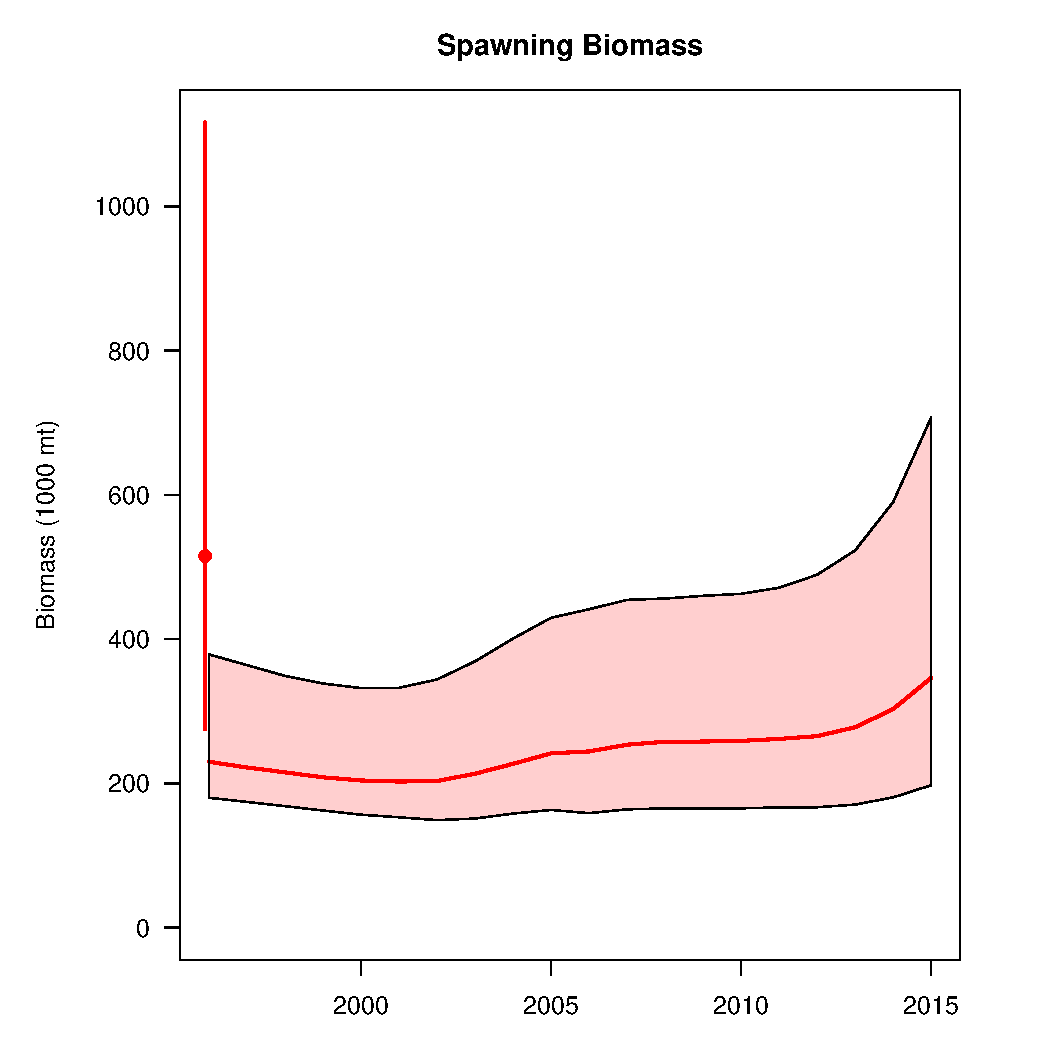
\includegraphics[width=\maxwidth]{C:/github/csas-latex/doc/figure/figBaseSpawnBioMCMC} \caption[Spawning biomass for the base model MCMC run]{Spawning biomass for the base model MCMC run.\label{fig:figBaseSpawnBioMCMC}}
\end{figure}

\begin{kframe}\begin{verbatim}
## [1] TRUE
\end{verbatim}
\end{kframe}
\end{knitrout}


%plotTS(scenario=1,plotNum=1,savefig=FALSE,plotMCMC=FALSE,ci=ci,burnthin=list(1000,0),burnthin,ps=ps,leg='topright')
%<<figSpawnBioMCMC, fig.pos='t', fig.height=4, fig.width=4, fig.cap='Spawning Biomass MCMC'>>=
%mydata  <-  data.frame(aa = 1:10, bb  <-  10:1)
%plot(mydata$aa, mydata$bb)
%@

%plotTS(scenario=1,plotNum=1,savefig=FALSE,plotMCMC=FALSE,ci=ci,burnthin=burnthin,ps=ps,leg='topright')

%<<fig1, out.width='.5\\linewidth', fig.align='center', fig.cap="Spawning biomass of base scenario.", fig.pos='h!'>>=
%plot(1:10,1:10)
%@

\newpage



%\rfoot{Appendix B -- Catch Data}
%\input{app-catch/app-catch}

%\rfoot{Appendix C -- Trawl Surveys}
%\input{app-surveys/app-surveys}

%\rfoot{Appendix C -- CPUE Analyses}
%% CPUE.tex

\clearpage

\chapter{Standardisation of Commercial Trawl CPUE}

\section{Introduction}

Commercial catch and effort data have been used to generate indices of abundance in several ways. The simplest indices are derived from the arithmetic mean or geometric mean of catch divided by an appropriate measure of effort (Catch Per Unit Effort or CPUE) but such indices make no adjustments for changes in fishing practices or other non-abundance factors which may affect catch rates. Consequently, methods to standardise for changes to vessel configuration, the timing or location of catch and other possible effects have been developed to remove potential biases to CPUE that may result from such changes. In these models, abundance is represented as a“year effect”and the dependent variable is either an explicitly calculated CPUE represented as catch divided by effort, or an implicit CPUE represented as catch per tow or catch per record. In the latter case, additional effort terms can be offered as explanatory variables, allowing the model to select the effort term with the greatest explanatory power. It is always preferable to standardise for as many factors as possible when using CPUE as a proxy for abundance. Unfortunately, it is often not possible to adjust for factors that might affect the behaviour of fishers, particularly economic factors, resulting in indices that may not entirely reflect the underlying stock abundance.

\section{Methods}
\subsection{Arithmetic and Unstandardised CPUE}

Arithmetic and unstandardised CPUE indices provide potential measures of relative abundance, but are generally considered unreliable because they fail to take into account changes in the fishery, including spatial and temporal changes as well as behavioural and gear changes. They are frequently calculated because they provide a measure of the overall effect of the standardisation procedure.

Arithmetic CPUE $\left(\hat{A}_y\right)$ in year $y$ was calculated as the total catch for the year divided by the total effort in the year using equation~\ref{eq:cpueArith}:

\begin{align} \label{eq:cpueArith}
\hat{A}_y=\bM{\frac{\sum\limits_{i=1}^{n_y}{C_{i,y}}}{\sum\limits_{i=1}^{n_y}{E_{i,y}}}}
\end{align}
\begin{addmargin}[3em]{1em}
where $C_{i,y}$ is the catch, $E_{i,y}=T_{i,y}$ (tows) or $E_{i,y}=H_{i,y}$ (hours fished) for record $i$ in year $y$, and $n_y$ is the number of records in year $y$.
\end{addmargin}

Unstandardised (geometric) CPUE assumes a log-normal error distribution. An unstandardised index of CPUE $\left(\hat{G}_y\right)$ in year y was calculated as the geometric mean of the ratio of catch to effort for each record i in year y using  equation~\ref{eq:cpueGeom}:

\begin{align} \label{eq:cpueGeom}
\bM{\hat{G}_y=\bM{e^{\frac{\sum\limits_{i=1}^{n_y}{ln{\frac{C_{i,y}}{E_{i,y}}}}}{n_y}}}}
\end{align}
\begin{addmargin}[3em]{1em}
where $C_{i,y}$, $E_{i,y}$, and $n_y$ are as defined for equation~\ref{eq:cpueArith}.
\end{addmargin}

\subsection{Standardised CPUE}

These models are preferred over the unstandardised models described above because they can account for changes in fishing behaviour and other factors which may affect the estimated abundance trend, as long as the models are provided with adequate data. In the models described below, catch per record is used as the dependent variable and the associated effort is treated as an explanatory variable.

\subsubsection{Lognormal Model}

Standardised CPUE assumes a lognormal error distribution, with explanatory variables to used represent changes in the fishery. A standardised CPUE index (Eq.~\ref{eq:cpueLognormal}) is calculated from a generalised linear model (GLM) (\citet{qd99}) using a range of explanatory variables including [year], [month], [depth], [vessel] and other available factors:

\begin{align} \label{eq:cpueLognormal}
\bM{ln(I_i)=B+Y_{y_i}+\alpha_{a_i}+\beta_{b_i}+...+f(\chi_i)+f(\delta_i)+...+\varepsilon_i}
\end{align}
\begin{addmargin}[3em]{1em}
where $I_i=C_i$ (where: $B$ is the intercept; $Y_{y_i}$ is the year coefficient for the year corresponding to the $i$th record; $\alpha_{a_i}$ and $\beta_{b_i}$ are the coefficients for factorial variables $a$ and $b$ corresponding to the $i$th record; $f(\chi_i)$ and $f(\delta_i)$ are polynomial functions (to the 3\textsuperscript{rd} order) of the continuous variables $\chi_i$ and $\delta_i$ corresponding to the $i$th record; and $\varepsilon_i$ is an error term.
\end{addmargin}

The actual number of factorial and continuous explanatory variables in each model depends on the model selection criteria. Because each record represents a single tow, $C_i$ has an implicit associated effort of one tow. Hours fished for the tow is represented on the right-hand side of the equation, usually as a continuous (polynomial) variable.

Note that calculating standardised CPUE with Eq.~\ref{eq:cpueLognormal} without additional explanatory variables is equivalent to using Eq.~\ref{eq:cpueGeom}, provided the same definition for  is used.

Canonical coefficients and standard errors were calculated for each categorical variable (\citet{francis1999}). Standardised analyses typically set one of the coefficients to 1.0 without an error term and estimate the remaining coefficients and the associated error relative to the fixed coefficient. This is required because of parameter confounding. The \citet{francis1999} procedure rescales all coefficients so that the geometric mean of the coefficients is equal to 1.0 and calculates a standard error for each coefficient, including the fixed coefficient.

Coefficient-distribution-influence plots (CDI plots) are visual tools to facilitate understanding of patterns which may exist in the combination of coefficient values, distributional changes, and annual influence (\citet{bentley2011}). CDI plots were used to illustrate each explanatory variable added to the model.

\subsubsection{Binomial Logit Model}

The procedure described by Eq.~\ref{eq:cpueLognormal} is necessarily confined to the positive catch observations in the data set because the logarithm of zero is undefined. Observations with zero catch were modelled by fitting a logit regression model based on a binomial distribution and using the presence/absence of \fishname as the dependent variable (where 1 is substituted for $ln(I_i)$ in Eq.~\ref{eq:cpueLognormal} if it is a successful catch record and 0 if it is not successful) and using the same data set. Explanatory factors are estimated in the model in the same manner as described in Eq.~\ref{eq:cpueLognormal}. Such a model provides an alternative series of standardised coefficients of relative annual changes that is analogous to the series estimated from the lognormal regression.

\subsubsection{Combined Model}

A combined model, integrating the two sets of relative annual changes estimated by the lognormal and binomial models, can be estimated using the delta distribution, which allows zero and positive observations (\citet{vignaux1994}). Such a model provides a single index of abundance which integrates the signals from the positive (lognormal) and binomial series. This approach uses the following equation to calculate an index based on the two contributing indices:

\begin{align} \label{eq:cpueGeom}
\bM{^CY_y=\frac{^LY_y}{\left(1-P_0\left(1-\frac{1}{^BY_y}\right)\right)}}
\end{align}
\begin{addmargin}[3em]{1em}
where $^cY_y$ = combined index for year $y$, $^LY_y$ = lognormal index for year $I$, $^BY_y$ = binomial index for year $I$, and $P_0$ is the proportion zero for base year $0$. 
\end{addmargin}

\citet{francis2001} suggests that a bootstrap procedure is the appropriate way to estimate the variability of the combined index. Therefore, confidence bounds for the combined model were estimated using a bootstrap procedure based on 500 replicates, drawn with replacement.

\subsection{Preliminary inspection of the data}

Three separate but similar analyses are reported in this Appendix. Each are tow-by-tow analyses for combined DFO major areas using total catch (landings + discards) confined to the period 1996–2013, the period when detailed positional data for every tow are available and when there are estimates of discarded catch for the tow, because of the presence of an observer on board the vessel. These data are held in the DFO PacHarvestTrawl (PacHarv) and GFFOS databases (Fisheries and Oceans Canada, Pacific Region, Groundfish Data Unit);

Tow-by-tow catch and effort data for \fishname\ from the BC bottom trawl fishery operating off the west coast of Vancouver Island (WCVI: Areas 3C and 3D) or Queen Charlotte Strait (Areas 5A and 5B) or Hecate Strait and Dixon Entrance (Areas 5C and 5D) from 1996 to 2013 were selected using the following criteria:

\begin{itemize}
  \item{Tow start date between 1 January 1996 and 31 December 2013}
  \item{Bottom trawl type (includes soft and hard bottom trawl types after 2006) (includes ‘unknown’ gear)}
  \item{Fished in PMFC regions: 3C and 3D, or 5A and 5B, or 5C and 5D (depending on the analysis)}
  \item{Fishing success code $\leq$ 1 (code 0= unknown; code 1= useable)}
  \item{Catch of at least one fish or invertebrate species (no water hauls or inanimate object tows )}
  \item{Valid depth field}
  \item{Valid latitude and longitude co-ordinates}
  \item{Valid estimate of time towed that was greater than 0 hours and less than or equal to 6 hours}
\end{itemize}

Each record represents a single tow, which results in equivalency between the number of records and number of tows. Catch per record can therefore be used to represent CPUE, because each record (tow) has an implicit effort component. Table~\ref{tab:cpueTripsDepths} shows the empirical 1\% and 99\% quantiles of the distribution of depths for tows which captured \fishname\ in each of the three analyses. The bounding depths used in each analysis are also shown.

It is possible that the deeper recorded depths are in error or document tows that passed through a wide range of depths because the tow depth is taken from the depth recorded at the beginning of the tow (the field which is most commonly populated).

Vessels which only fished occasionally in each area or which did not actively fish \fishname\ were excluded from these analyses by setting minimum qualification criteria based on the number of trips per year and number of years fishing. A further restriction of stipulating a minimum number of successful tows was imposed in the 3CD and 5AB analyses. This was done to further reduce the number of qualifying vessels and to ensure that there were sufficient data to characterise the core fleet. This was not done for the 5CD analysis because of the small number of core vessels and the relatively large number of available qualifying tows for each vessel. Vessels which met the minimum criteria were included in the core vessel fleet, with all data for a qualifying vessel included, regardless of the number of trips in any year, once the vessel had been selected. Table~\ref{tab:cpueTripsQualify} gives the total number of vessels in each analysis, the number of qualifying trips per year, the number of years required and the minimum number of successful tows (if applicable). The final size of the core fleet is also given, as well as the proportion of the total fleet catch included in the analysis. Note that, in the 3CD analysis, one vessel was dropped because of uncertainties associated with the data. This vessel accounted for nearly 11,000 t of the total 60,700 t of catch in the dataset, with this amount of catch taken with just over 530 tows and about 500 hours of fishing. When this vessel was included in the analysis, its CPUE was approximately 60 times greater than the average for the rest of the fleet. The reason for this discrepancy is not known, but this vessel was dropped from the analysis, given its substantial difference from the remainder of the data. However, the removal of this vessel from the analysis had almost no effect on the estimated year indices.

Each of the figure references in table~\ref{tab:cpueTripsQualify} show the relationship of the two qualifying criteria with the resulting number of vessels and the proportion of catch retained in the analysis. The “bubble plot” references show the degree of vessel overlap across years for each analysis, with the requirement that the vessel data need to overlap in order for the model to correctly interpret the vessel and year categorical variables. These plots show that the overlap was good in all three models, with an adequate number of vessels operating across the 18 years of data. Only tows which were less than 6 hours long were used in the analyses. This criterion dropped very little data because 98\% to 99\% of the tows took less than 6 hours, depending on the analysis. The final data sets are large, ranging from about 30,000 to nearly 60,000 successful tows and 27,800 t to 40,000 t of total \fishname\ catch (Table~\ref{tab:cpueCatchRate}).

The explanatory variables found in table~\ref{tab:cpueExplanatory}  were offered to the model, based on the tow-by-tow information in each record.

\section{Results}

\subsection{3CD Tow-by-tow Analysis}

\subsubsection{Lognoirmal Positive Model}


\begin{table}[b]
%\tiny
\centering
\caption{\label{tab:cpueTripsDepths} Trips which qualify for the CPUE analyses. Vessels which did not actively fish \fishname\ were excluded by the criteria number of trips per year and number of years fishing.}
\begin{tabular}{lrrrrrl}
\hline
\specialcell{Analysis\\area} & 1\% (m) & 99\% (m) & \specialcell{Lower bound\\used} & \specialcell{Upper bound\\used} & \specialcell{\#depth\\bins} & Figure ref. \\
\hline
3CD & 71 & 750 & 60 & 760 & 18 & FIGREF \\
5AB & 64 & 439 & 40 & 460 &    & FIGREF \\
5CD & 39 & 388 & 20 & 400 & 10 & FIGREF \\
\hline
\end{tabular}
\end{table}


\begin{table}[b]
%\tiny
\centering
\caption{\label{tab:cpueTripsQualify} Trips which qualify for the CPUE analyses. Vessels which did not actively fish \fishname\ were excluded by the criteria number of trips per year and number of years fishing.}
\begin{tabular}{lrrrrrrll}
\hline
\specialcell{Analysis\\area} & \specialcell{Total\\vessels} & \specialcell{\#qualifying\\trips/year} & \specialcell{\#qualifying\\years} & \specialcell{Minimum \#\\tows} & \specialcell{\#qulifying\\vessels} & \specialcell{\% total\\catch} & Figure ref. & Bubble plot \\
\hline
3CD & 101 & 4 & 4 & 299 & 37 & 66\textsuperscript1 & FIGREF & FIGREF \\
5AB & 109 & 4 & 4 & 292 & 44 &                  79 & FIGREF & FIGREF \\
5CD &  91 & 5 & 5 &   0 & 18 &                  82 & FIGREF & FIGREF \\
\hline
\end{tabular}
\textsuperscript1After dropping the anomalous vessel described in the text
\end{table}

\begin{table}[b]
%\tiny
\centering
\caption{\label{tab:cpueCatchRate} Catch rates by area for \fishname\ }
\begin{tabular}{lrr|rr|lrr}
\hline
    &  &  & \multicolumn{2}{|r|}{Mean Catch Rate} \\
\specialcell{Analysis\\area} & \#tows & \specialcell{Total ARF\\catch (t)} & kg/tow & kg/h & \specialcell{Summary\\table ref.} & \specialcell{\#latitude\\bins} & \specialcell{\#locality\\bins} \\
\hline
3CD & 41,600 & 40,300 & 921 & 443 & TABREF & 22 & 27 \\
5AB & 57,900 & 33,200 & 534 & 250 & TABREF & 18 & 19 \\
5CD & 30,700 & 27,800 & 853 & 471 & TABREF & 22 & 21 \\
\hline
\end{tabular}
\end{table}

\begin{table}[b]
%\tiny
\centering
\caption{\label{tab:cpueExplanatory} Explanatory variables used in the model.}
\begin{tabular}{ll}
\hline
Year (1 January - 31 December) & 18 categories \\
\hline
Hours fished & continuous: 3rd order polynomial \\
\hline
Month & 12 categories\\
\hline
Latitude separated in 0.1° bands beginning with 48°N & \specialcell{variable for each analysis (see table~\ref{tab:cpueCatchRate})\\includes a final aggregated category} \\
\hline
DFO locality (Rutherford 1995) & \specialcell{variable for each analysis (see table~\ref{tab:cpueCatchRate})\\includes a final aggregated category} \\
\hline
Vessel & variable for each analysis (see table~\ref{tab:cpueCatchRate}) \\
\hline
Depth aggregated into 40 m depth bands & variable for each analysis (see table~\ref{tab:cpueCatchRate}) \\
\hline
DFO Major region & 2 categories for each analysis \\
\hline
\end{tabular}
\end{table}


\clearpage


%\setcounter{page}{68}

%\rfoot{Appendix E -- Age Data}
%\input{app-biology/app-agesrev}

%\rfoot{Appendix G -- Results}
%\input{app-results/app-results}

%\rfoot{Appendix H -- Habitat}
%\input{app-habitat/app-habitat}

%\rfoot{Appendix I -- Sensitivities}
%\input{app-sensitivities/app-sensitivities}

\end{document}
